\chapter{Étude de la méthode}
    \label{chapter:4-ETUDES}
	
	% RÉSUMÉ DES ÉPISODES PRÉCÉDENTES:
	Dans le chapitre précédent, nous avons présenté une méthode de création d'un jeu de données d'entrainement pour un assistant conversationnel, que nous appelons "\textit{clustering interactif}" :
	\begin{todolist}
	    % 1. Structure de la méthode.
		\item[\itemok] La méthode proposée repose sur la combinaison entre un regroupement automatique des données par la machine et l'annotation de contraintes binaires par un expert métier pour corriger le regroupement proposé ;
		% 2. Enjeu 1 de la méthode : moins de technique.
		\item[\itemok] Une telle approche devrait limiter les pré-requis techniques actuellement exigés à un expert métier en les déléguant à la machine.
		% 2. Enjeu 2 de la méthode : plus de connaissance métier.
		\item[\itemok] En échange, l'expert se concentre d'avantage sur la transmission de ses connaissances avec une annotation caractérisant la similitude métier entre deux données.
		% 3. Divers.
		\item[\itemok] ...\todo{divers à compléter (technique ? méthode ? ...).}
	\end{todolist}
	
	% ANNONCE DU BUT DU CHAPITRE: TEST DE LA MÉTHODE.
	Comme nous l'avons détaillé dans le chapitre~\ref{chapter:2-ETAT-DE-L-ART}, des procédés d'annotation similaires existent pour des données facilement visualisables, comme dans le cadre du traitement d'images. Cependant, l'application d'une telle approche dans le cadre de la classification de données textuelles est peu détaillée dans la littérature. Ainsi, dans cette partie, nous étudierons la faisabilité d'un \textit{clustering interactif} pour des données textuelles en explorant les questions suivantes :
	\begin{todolist}
		% 1. Efficacité.
		\item Peut-on obtenir une base d'apprentissage à l'aide de notre proposition d'implémentation de la méthodologie d'\textit{clustering} interactif ? (cf. hypothèse d'\textbf{efficacité} en section~\ref{section:4.1-HYPOTHESE-EFFICACITE})
		% 2. Efficience.
		\item Peut-on déterminer un paramétrage optimal de cette implémentation pour obtenir plus rapidement une base d'apprentissage ? (cf. hypothèse d'\textbf{efficience} en section~\ref{section:4.2-HYPOTHESE-EFFICIENCE})
		% 3. Pertinence.
		\item A un instant donné, peut-on estimer la pertinence métier d'une base d'apprentissage en cours de construction ? (cf. hypothèse de \textbf{pertinence} en section~\ref{section:4.3-HYPOTHESE-PERTINENCE})
		% 4. Coûts.
		\item D'après les données initiales, peut-on approximer l'investissement nécessaire pour obtenir une base d'apprentissage exploitable ? (cf. hypothèse sur les \textbf{coûts} en section~\ref{section:4.4-HYPOTHESE-COUTS})
		% 5. Impact.
		\item A un instant donné, peut-on estimer les gains potentiels d'une nouvelle étape de raffinage de la base d'apprentissage en cours de construction ? (cf. hypothèse d'\textbf{impact} en section~\ref{section:4.5-HYPOTHESE-IMPACT})
		% 6. Robustesse.
		\item Peut-on estimer l'influence d'une erreur ou d'une différence d'annotation dans la construction de la base d'apprentissage ? (cf. hypothèse de \textbf{robustesse} en section~\ref{section:4.6-HYPOTHESE-ROBUSTESSE})
	\end{todolist}
	
	% ILLUSTRATION: SCHEMA DES HYPOTHESES
	Afin d'illustrer ces interrogations, nous vous proposons de considérer de la figure~\ref{figure:HYPOTHESE-00-DEFAULT}. Dans les sections suivantes, cette figure évoluera pour résumer les études réalisées.
	
	\begin{figure}[H]
		\centering
		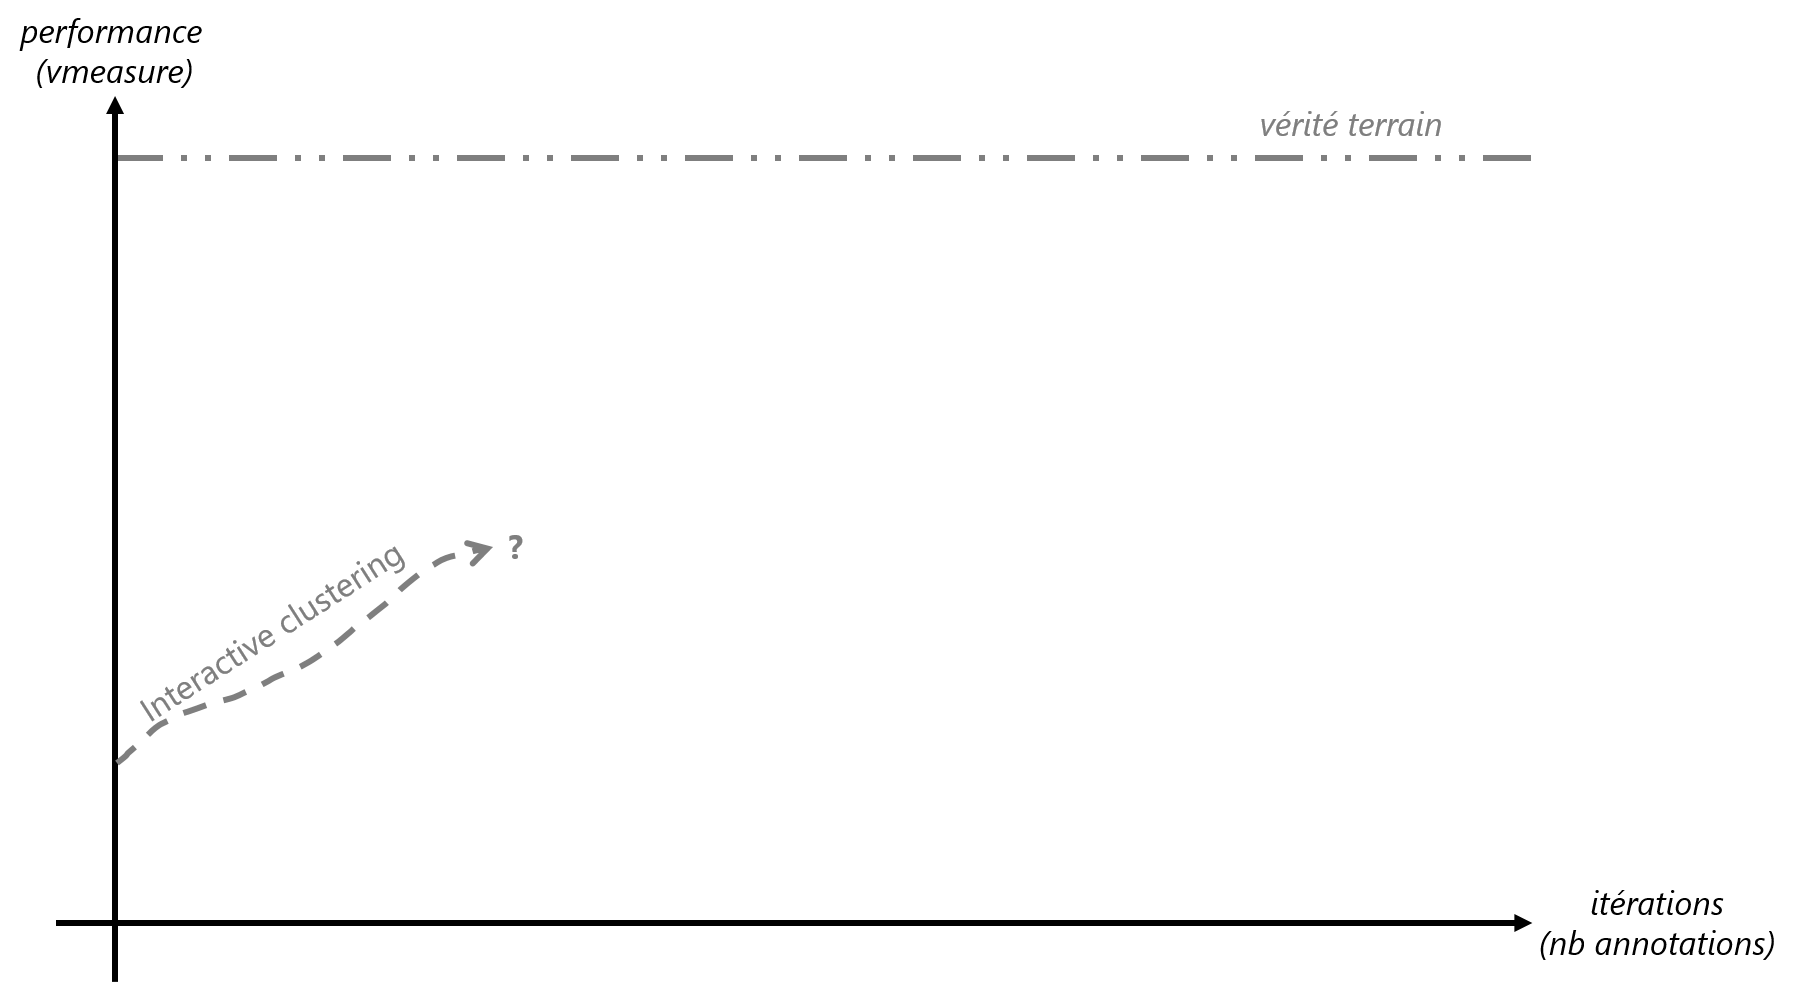
\includegraphics[width=0.8\textwidth]{figures/hypotheses-00-default}
		\caption{Illustration des études réalisées sur le \textit{clustering} interactif (\textit{étape 0/6}) en schématisant l'évolution de la performance (\textit{v-measure par rapport à une vérité terrain}) d'une base d'apprentissage en cours de construction en fonction du nombre d'itérations de la méthode (\textit{nombre d'annotations}).}
		\label{figure:HYPOTHESE-00-DEFAULT}
	\end{figure}
	
	% PRÉAMBULE TECHNIQUE : CPU + scrips + datasets.
	Pour ces études, l'exécution des différentes expériences a été réalisée sur des CPU \textit{Intel(R) Xeon(R) CPU E5-2660 v4 \@ 2.00GHz} et parallélisé avec la librairie Python \textit{multiprocessing} (un worker par CPU).
	Les scripts d'exécution et d'analyse de ces expériences, rédigés au sein de notebooks Python et/ou R, sont disponibles dans~\cite{schild:cognitivefactory-interactive-clustering-comparative-study:2021}.
	Enfin, les jeux de données utilisés pour ces études sont détaillés en Annexe~\ref{annex:C-ANNEXE-DATASET}.
	
	
	% TABLE DES MATIÈRES DU CHAPITRE
    \minitoc

    %%%%%--------------------------------------------------------------------
    %%%%% Section 4.1: Hypothèse d'efficacité.
    %%%%%--------------------------------------------------------------------
    \section{Hypothèse d'efficacité : « \textit{est-ce que la méthode fonctionne ?} »}
	\label{section:4.1-HYPOTHESE-EFFICACITE}
	
		%%% Formulation des hypothèses:
		Nous aimerions vérifier l'hypothèse d'efficacité suivante :
		\todo{à compléter}

		\begin{tcolorbox}[
			title=\textbf{Hypothèse d'efficacité},
			colback=gray!20,
			colframe=gray!50!black!75,
			width=\linewidth
		]
			« Une méthodologie d'annotation basée sur le \textit{clustering} interactif \textbf{peut converger} vers une vérité terrain préalablement établie (cf. figure~\ref{figure:HYPOTHESE-EFFICACITE}. »
			
			\begin{figure}[H]
				\centering
				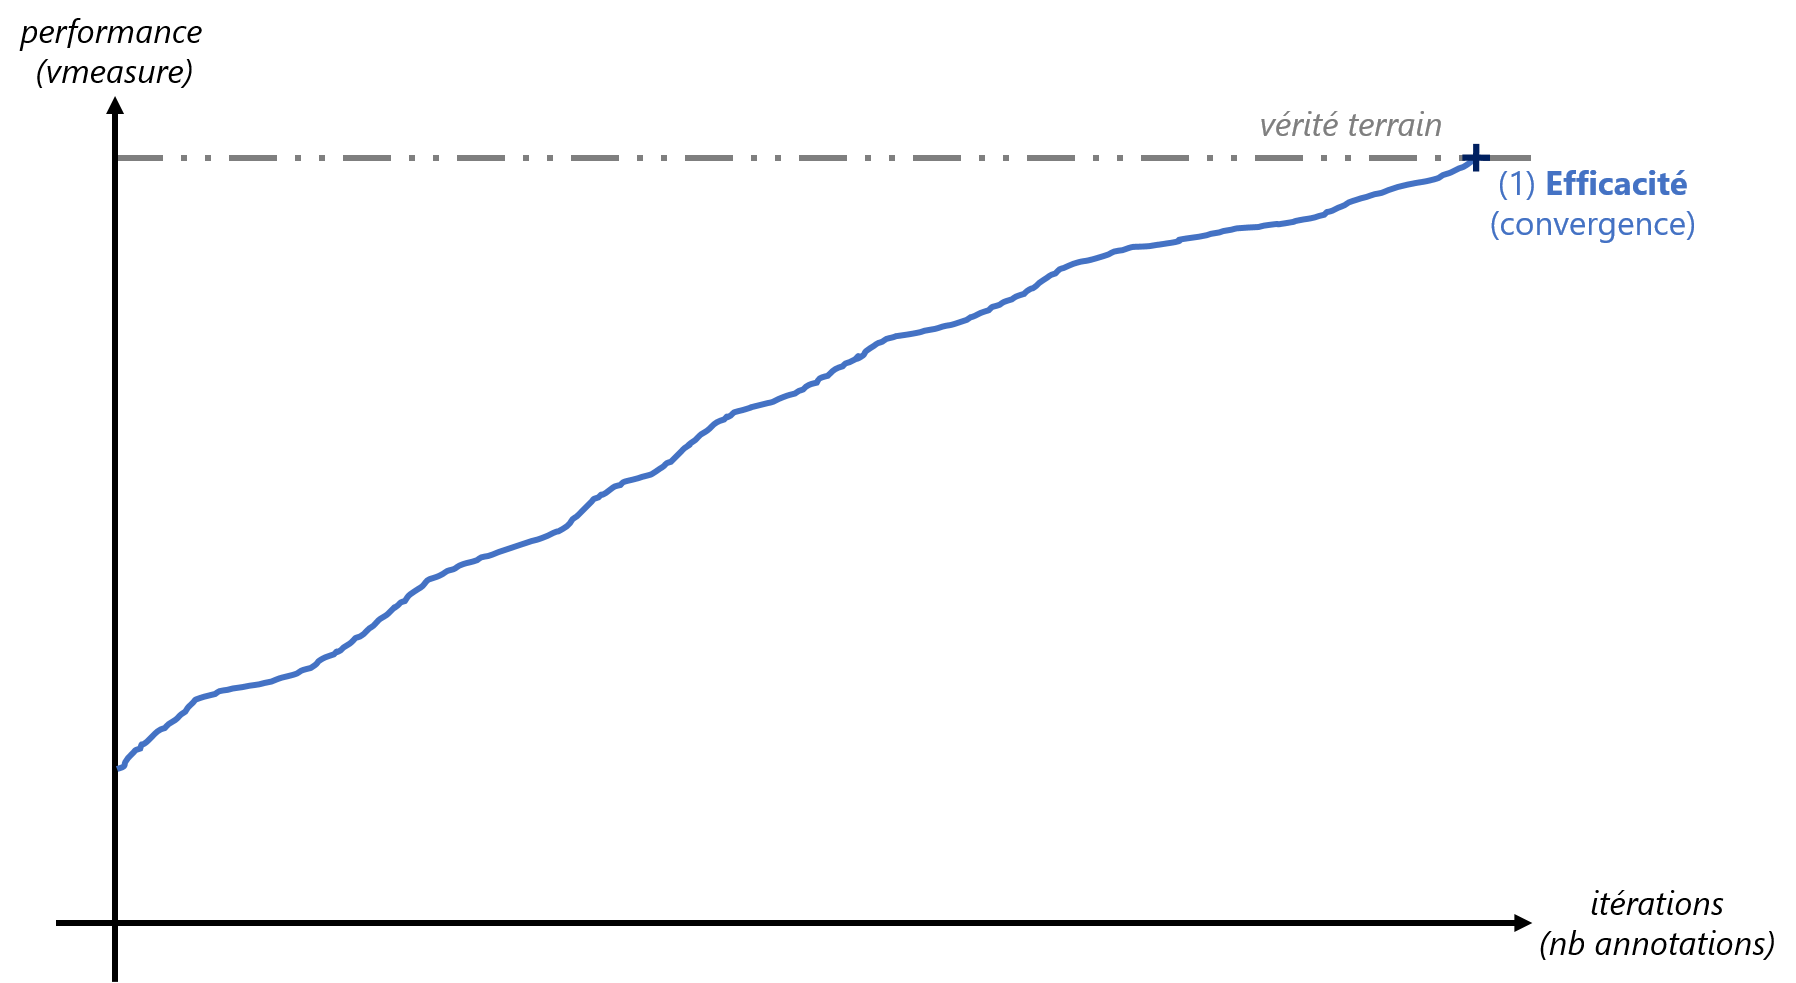
\includegraphics[width=0.8\textwidth]{figures/hypotheses-01-efficacite}
				\caption{Illustration des études réalisées sur le \textit{clustering} interactif (\textit{étape 1/6}) en schématisant l'évolution de la performance (\textit{v-measure par rapport à une vérité terrain}) d'une base d'apprentissage en cours de construction en fonction du nombre d'itérations de la méthode (\textit{nombre d'annotations}).}
				\label{figure:HYPOTHESE-EFFICACITE}
			\end{figure}

		\end{tcolorbox}
		
		%%%
		%%% Subsection 4.1.1: Étude de convergence
		%%%
		\subsection{Étude de convergence}
	
			%%% Protocole expérimental.
			\subsubsection{Protocole expérimental}
				\todo[inline]{Description succincte du protocole expérimental dans l'encadré d'hypothèse ?}
			
				% Description rapide du protocole.
				Pour vérifier l'hypothèse d'efficacité, nous proposons une simulation de création d'un jeu d’entraînement d'un assistant conversationnel en employant notre méthodologie d'annotation basée sur le \textit{clustering} interactif.
				Pour cela, nous ré-annotons une version non labellisée d'une vérité terrain à disposition, en commençant sans aucune contrainte et en terminant lorsque toutes les contraintes possibles entre les données soient annotées.
				
				% Description de la simulation de l'annotation.
				Pour simuler l'annotation de l'expert métier entre deux données, nous utilisons la comparaison des labels de la vérité terrain : ainsi, deux données auront une contrainte \textit{MUST-LINK} si elles ont le même label, et une contrainte \textit{CANNOT-LINK} sinon. Cela traduit le prérequis d'avoir un annotateur qui soit capable de caractériser la similitude entre deux données.
				
				% Description implémentation de l'interactive clustering.
				\todo{Description implémentation de l'interactive clustering (au préalable ?)}
				\todo{Description des paramètres testés}
				\todo{Description de l'évaluation}
				
				% Pseudo-code.
				La protocole expérimental est aussi décrit à l'aide du pseudo-code figurant dans Alg.~\ref{algorithm:4.1-PROTOCOLE-EXPERIMENTAL}.

				\begin{algorithm}
					\begin{algorithmic}[1]
						\Require données non segmentées, algorithmes et paramètres à tester
						\State \textbf{prétraitement}: suppression du bruits dans les données
						\State \textbf{vectorisation}: transformation des données en vecteurs
						\State \textbf{initialisation}: créer une liste vide de contraintes
						\State \textbf{clustering initial}: regrouper les données par similarité
						\State \textbf{évaluation}: comparer le clustering à la vérité terrain
						\Repeat
							\State \textbf{échantillonnage}: sélection de nouvelles contraintes à annoter
							\State \textbf{annotation}: simulation d'annotation en comparant les labels de la vérité terrain
							\State \textbf{clustering}: regrouper les données par similarité et avec les contraintes
							\State \textbf{évaluation}: comparer le clustering à la vérité terrain
						\Until{annotation de toutes les contraintes possibles}
						\Ensure données segmentées, toutes les contraints possibles sont annotées
					\end{algorithmic}
					\caption{Description en pseudo-code du protocole expérimental visant à estimer la faisabilité technique du clustering interactif.}
					\label{algorithm:4.1-PROTOCOLE-EXPERIMENTAL}
				\end{algorithm}

			%%% Résultats
			\subsubsection{Résultats obtenus}
				\todo[inline]{SECTION À RÉDIGER}
				
				\todo{max de clustering à itération 0}
				\todo{convergence}
				\todo{graphe évolution moyenne}

			%%% Discussion
			\subsubsection{Discussion}
				\todo[inline]{SECTION À RÉDIGER}
				
				\todo{convergence lente, mais convergence !}
				\todo{pas besoin d'une structure établie, mais de savoir distinguer}
				\todo{on peut optimiser (moyenne + écart-type itération convergence)}
	

    %%%%%--------------------------------------------------------------------
    %%%%% Section 4.2: Hypothèse d'efficience.
    %%%%%--------------------------------------------------------------------
    \section{Hypothèse d'efficience : « \textit{est-ce que l'implémentation est optimale ?} »}
	\label{section:4.2-HYPOTHESE-EFFICIENCE}
	
		%%% Formulation des hypothèses:
		Nous aimerions vérifier l'hypothèse d'efficience suivante :
		\todo{à compléter}

		\begin{tcolorbox}[
			title=\textbf{Hypothèse d'efficience},
			colback=gray!20,
			colframe=gray!50!black!75,
			width=\linewidth
		]
			« La vitesse de convergence du \textit{clustering} interactif \textbf{peut être optimisée} en réglant différents paramètres. Nous étudierons l'influence du prétraitement des données, de la vectorisation des données, de l'échantillonnage des contraintes à annoter et du \textit{clustering} sous contraintes (cf. figure~\ref{figure:HYPOTHESE-EFFICIENCE}. »
			
			
			\begin{figure}[H]
				\centering
				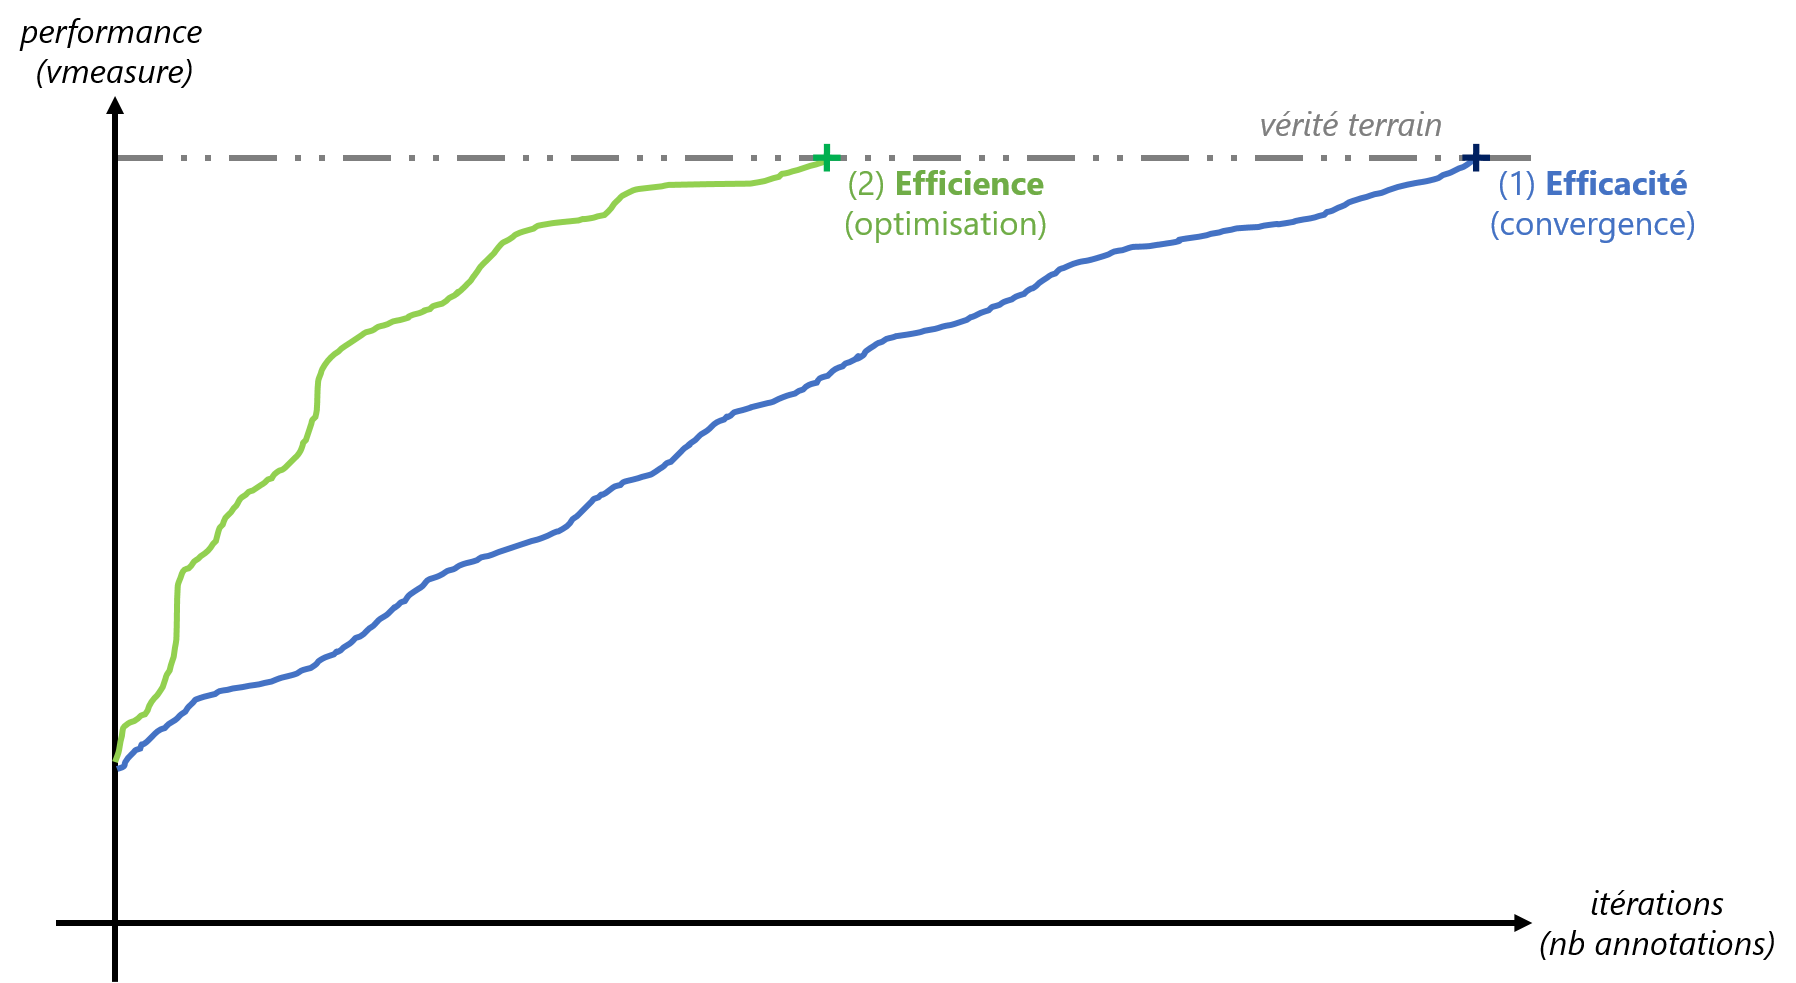
\includegraphics[width=0.8\textwidth]{figures/hypotheses-02-efficience}
				\caption{Illustration des études réalisées sur le \textit{clustering} interactif (\textit{étape 2/6}) en schématisant l'évolution de la performance (\textit{v-measure par rapport à une vérité terrain}) d'une base d'apprentissage en cours de construction en fonction du nombre d'itérations de la méthode (\textit{nombre d'annotations}).}
				\label{figure:HYPOTHESE-EFFICIENCE}
			\end{figure}

		\end{tcolorbox}
		
		%%%
		%%% Subsection 4.2.1: Étude des paramètres de convergence optimaux
		%%%
		\subsection{Étude des paramètres de convergence optimaux}
	
			%%% Protocole expérimental.
			\subsubsection{Protocole expérimental}
				\todo[inline]{Description succincte du protocole expérimental dans l'encadré d'hypothèse ?}
				\todo{Reprendre 4.1.1, mais pour estimer les meilleurs paramètres}
				\todo{seuils étudiés}
				\todo{ANOVA répété}

			%%% Résultats
			\subsubsection{Résultats obtenus}
				\todo{3 tableaux de paramètres}

			%%% Discussion
			\subsubsection{Discussion}
				\todo{meilleur paramétrage}
	

    %%%%%--------------------------------------------------------------------
    %%%%% Section 4.3: Hypothèse de pertinence.
    %%%%%--------------------------------------------------------------------
    \section{Hypothèse de pertinence : « \textit{est-ce le résultat est exploitable ?} »}
	\label{section:4.3-HYPOTHESE-PERTINENCE}
	
		%%% Formulation des hypothèses:
		Nous aimerions vérifier l'hypothèse de pertinence suivante :
		\todo{à compléter}

		\begin{tcolorbox}[
			title=\textbf{Hypothèse de pertinence},
			colback=gray!20,
			colframe=gray!50!black!75,
			width=\linewidth
		]
			« La vitesse de convergence du \textit{clustering} interactif \textbf{peut être optimisée} en réglant différents paramètres. Nous étudierons l'influence du prétraitement des données, de la vectorisation des données, de l'échantillonnage des contraintes à annoter et du \textit{clustering} sous contraintes (cf. figure~\ref{figure:HYPOTHESE-PERTINENCE}. »
			
			
			\begin{figure}[H]
				\centering
				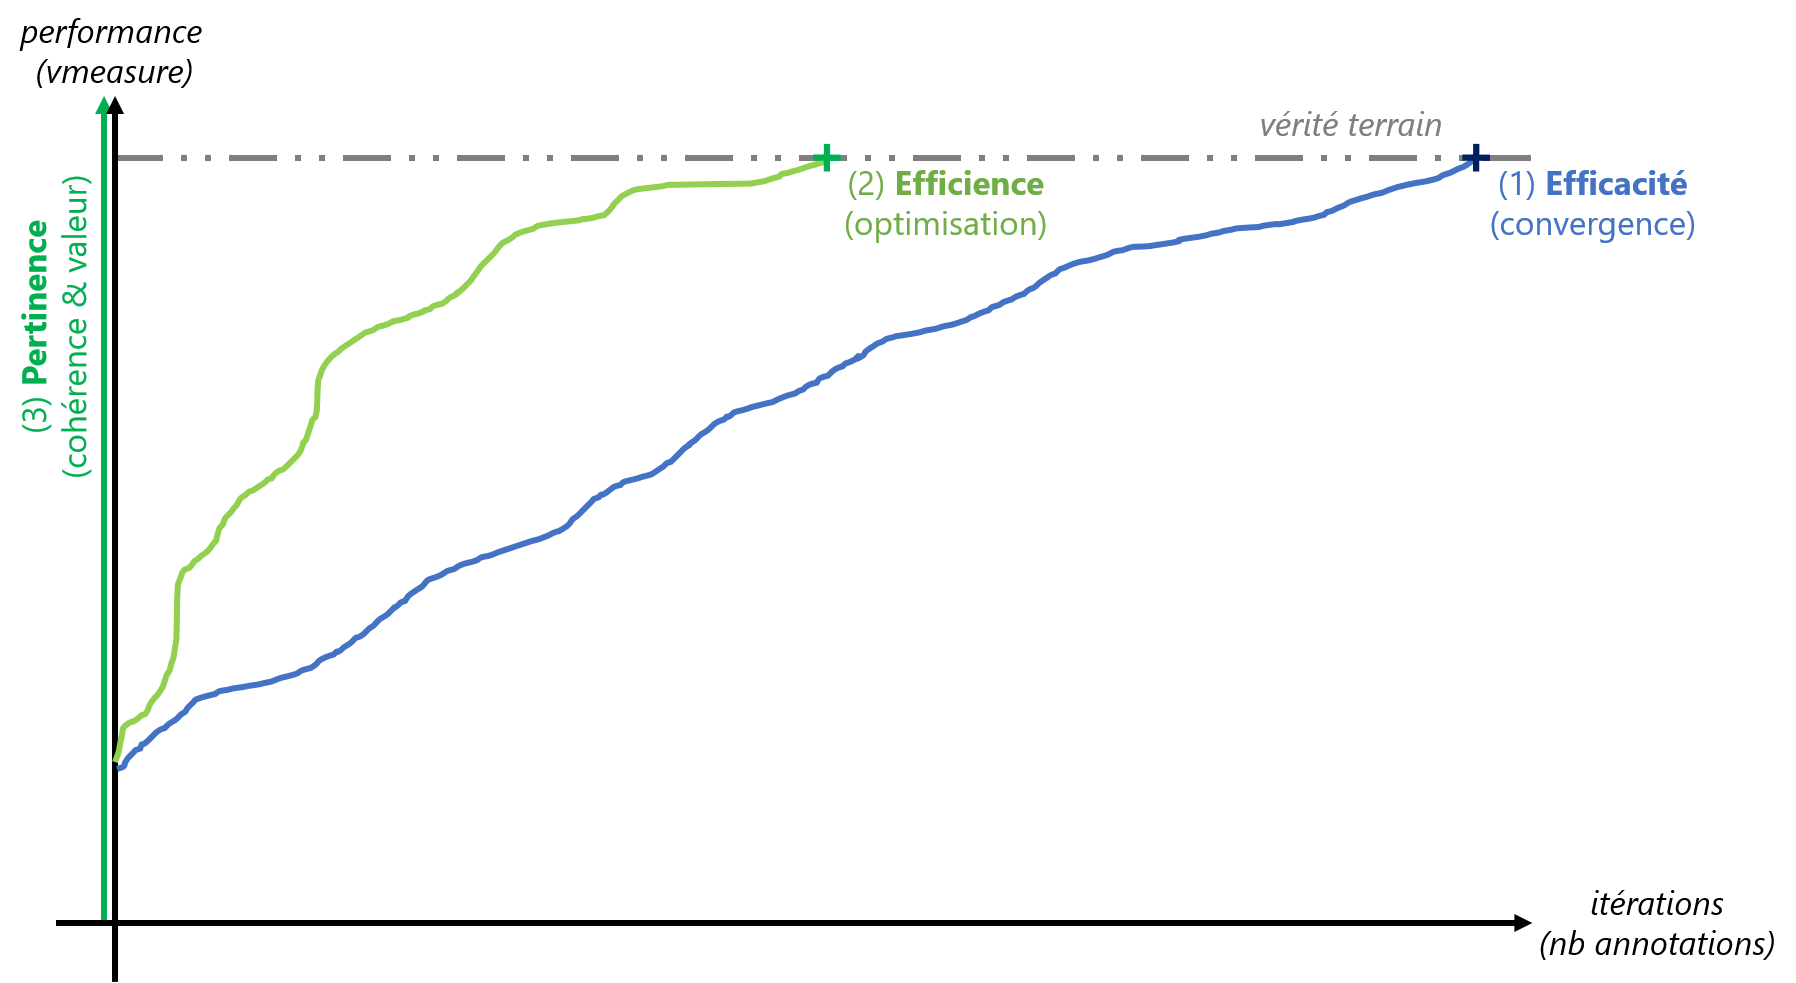
\includegraphics[width=0.8\textwidth]{figures/hypotheses-03-pertinence}
				\caption{Illustration des études réalisées sur le \textit{clustering} interactif (\textit{étape 3/6}) en schématisant l'évolution de la performance (\textit{v-measure par rapport à une vérité terrain}) d'une base d'apprentissage en cours de construction en fonction du nombre d'itérations de la méthode (\textit{nombre d'annotations}).}
				\label{figure:HYPOTHESE-PERTINENCE}
			\end{figure}

		\end{tcolorbox}
		
		%%%
		%%% Subsection 4.3.1: Étude de la cohérence statistique de la base d'apprentissage en cours de construction
		%%%
		\subsection{Étude de la cohérence statistique de la base d'apprentissage en cours de construction}
		
			%%% Protocole expérimental.
			\subsubsection{Protocole expérimental}
				\todo[inline]{Description succincte du protocole expérimental dans l'encadré d'hypothèse ?}

			%%% Résultats
			\subsubsection{Résultats obtenus}

			%%% Discussion
			\subsubsection{Discussion}
		
		%%%
		%%% Subsection 4.3.2: Étude de la pertinence sémentique de la base d'apprentissage en cours de construction
		%%%
		\subsection{Étude de la pertinence sémentique de la base d'apprentissage en cours de construction}
		
			%%% Protocole expérimental.
			\subsubsection{Protocole expérimental}
				\todo[inline]{Description succincte du protocole expérimental dans l'encadré d'hypothèse ?}

			%%% Résultats
			\subsubsection{Résultats obtenus}

			%%% Discussion
			\subsubsection{Discussion}
	

    %%%%%--------------------------------------------------------------------
    %%%%% Section 4.4: Hypothèse sur les coûts.
    %%%%%--------------------------------------------------------------------
    \section{Hypothèse sur les coûts : « \textit{combien dois-je investir ?} »}
	\label{section:4.4-HYPOTHESE-COUTS}
	
		%%% Formulation des hypothèses:
		Nous aimerions vérifier l'hypothèse sur les coûts suivante :
		\todo{à compléter}

		\begin{tcolorbox}[
			title=\textbf{Hypothèse sur les coûts},
			colback=gray!20,
			colframe=gray!50!black!75,
			width=\linewidth
		]
			« Il est possible de \textbf{mesurer le temps nécessaire} à une méthodologie d'annotation basée sur le \textit{clustering} interactif pour obtenir un résultat exploitable (cf. figure~\ref{figure:HYPOTHESE-COUTS}. »
			
			
			\begin{figure}[H]
				\centering
				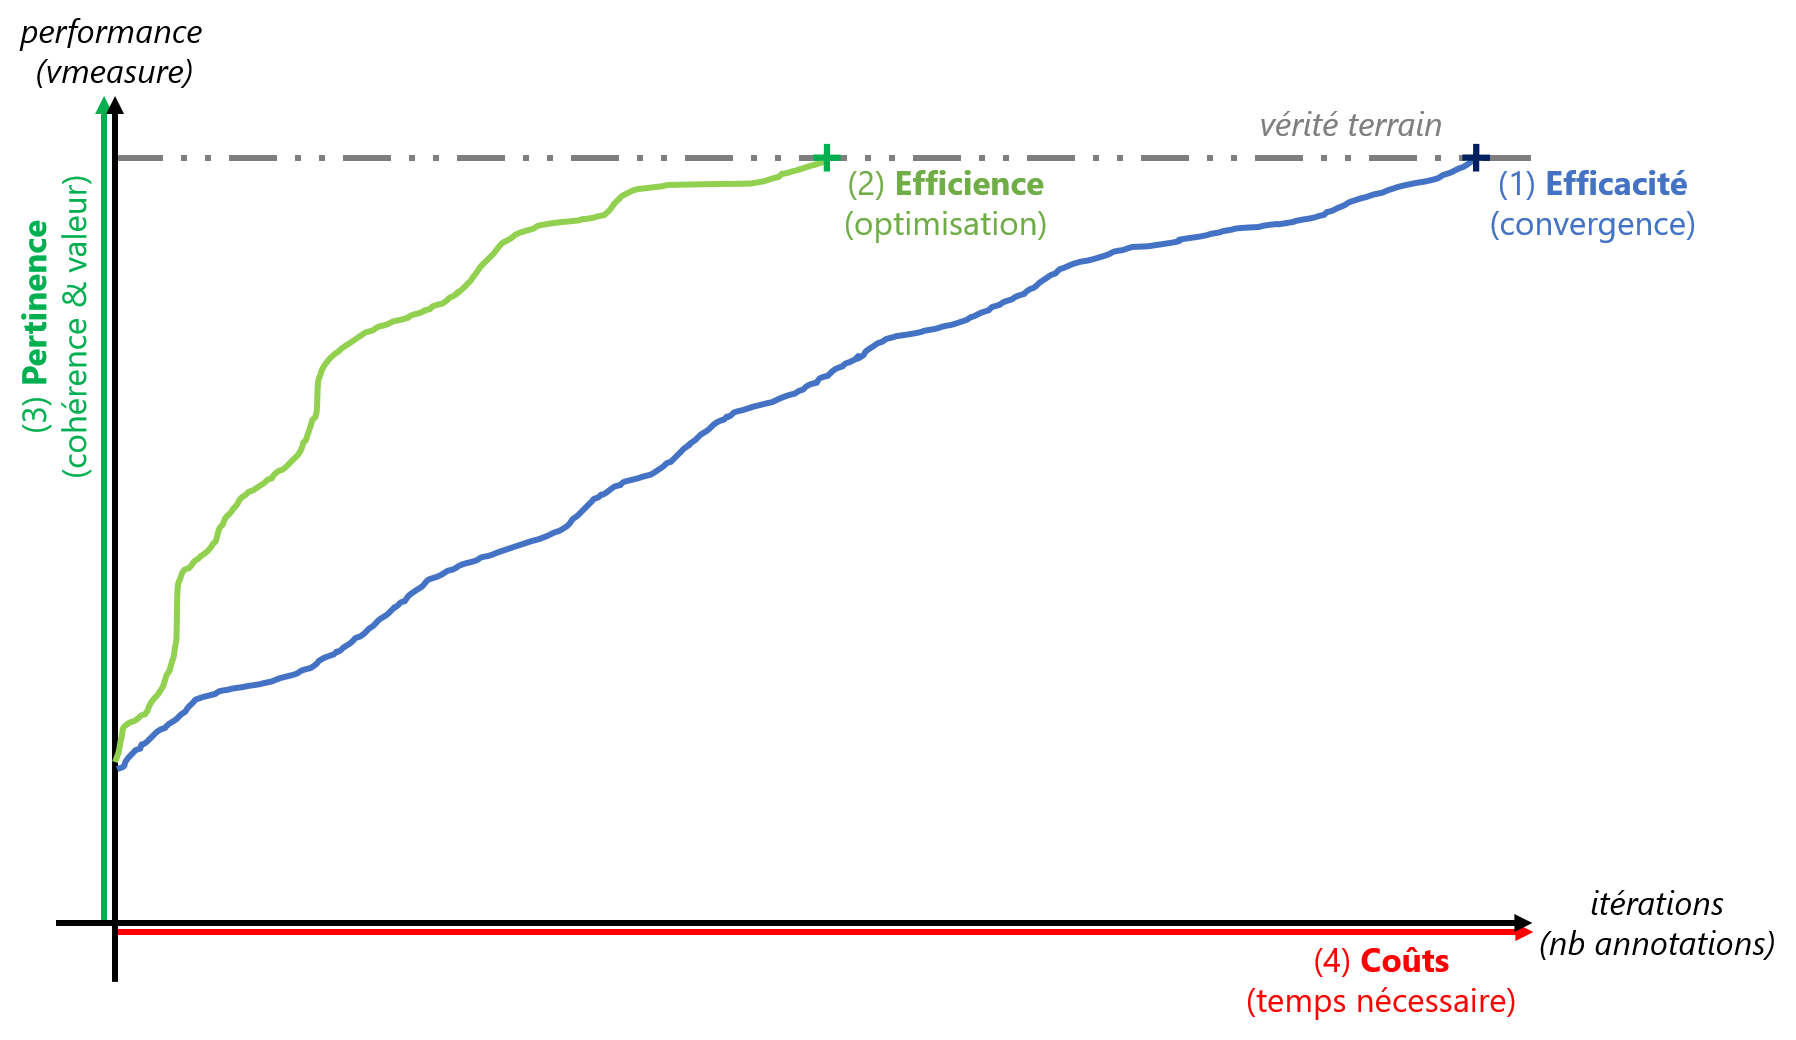
\includegraphics[width=0.8\textwidth]{figures/hypotheses-04-couts}
				\caption{Illustration des études réalisées sur le \textit{clustering} interactif (\textit{étape 4/6}) en schématisant l'évolution de la performance (\textit{v-measure par rapport à une vérité terrain}) d'une base d'apprentissage en cours de construction en fonction du nombre d'itérations de la méthode (\textit{nombre d'annotations}).}
				\label{figure:HYPOTHESE-COUTS}
			\end{figure}

		\end{tcolorbox}
		
		%%%
		%%% Subsection 4.4.1: Étude d'estimation du temps d'annotation par un expert métier
		%%%
		\subsection{Étude d'estimation du temps d'annotation par un expert métier}
		
			%%% Protocole expérimental.
			\subsubsection{Protocole expérimental}
				\todo[inline]{Description succincte du protocole expérimental dans l'encadré d'hypothèse ?}

			%%% Résultats
			\subsubsection{Résultats obtenus}

			%%% Discussion
			\subsubsection{Discussion}
		
		%%%
		%%% Subsection 4.4.2: Étude d'estimation du temps de calcul des algorithmes
		%%%
		\subsection{Étude d'estimation du temps de calcul des algorithmes}
		
			%%% Protocole expérimental.
			\subsubsection{Protocole expérimental}
				\todo[inline]{Description succincte du protocole expérimental dans l'encadré d'hypothèse ?}

			%%% Résultats
			\subsubsection{Résultats obtenus}

			%%% Discussion
			\subsubsection{Discussion}
		
		%%%
		%%% Subsection 4.4.3: Étude d'estimation du temps total d'un projet d'annotation
		%%%
		\subsection{Étude d'estimation du temps total d'un projet d'annotation}
		
			%%% Protocole expérimental.
			\subsubsection{Protocole expérimental}
				\todo[inline]{Description succincte du protocole expérimental dans l'encadré d'hypothèse ?}

			%%% Résultats
			\subsubsection{Résultats obtenus}

			%%% Discussion
			\subsubsection{Discussion}
	

    %%%%%--------------------------------------------------------------------
    %%%%% Section 4.5: Hypothèse d'impact.
    %%%%%--------------------------------------------------------------------
    \section{Hypothèse d'impact : « \textit{quel gain à chaque itération ?} »}
	\label{section:4.5-HYPOTHESE-IMPACT}
	
		%%% Formulation des hypothèses:
		Nous aimerions vérifier l'hypothèse d'impact :
		\todo{à reformuler}

		\begin{tcolorbox}[
			title=\textbf{Hypothèse d'impact},
			colback=gray!20,
			colframe=gray!50!black!75,
			width=\linewidth
		]
			« Il est possible d'estimer quand méthodologie d'annotation basée sur le \textit{clustering} interactif \textbf{a converger} vers un résultat satisfaisant (cf. figure~\ref{figure:HYPOTHESE-IMPACT}. »
			
			
			\begin{figure}[H]
				\centering
				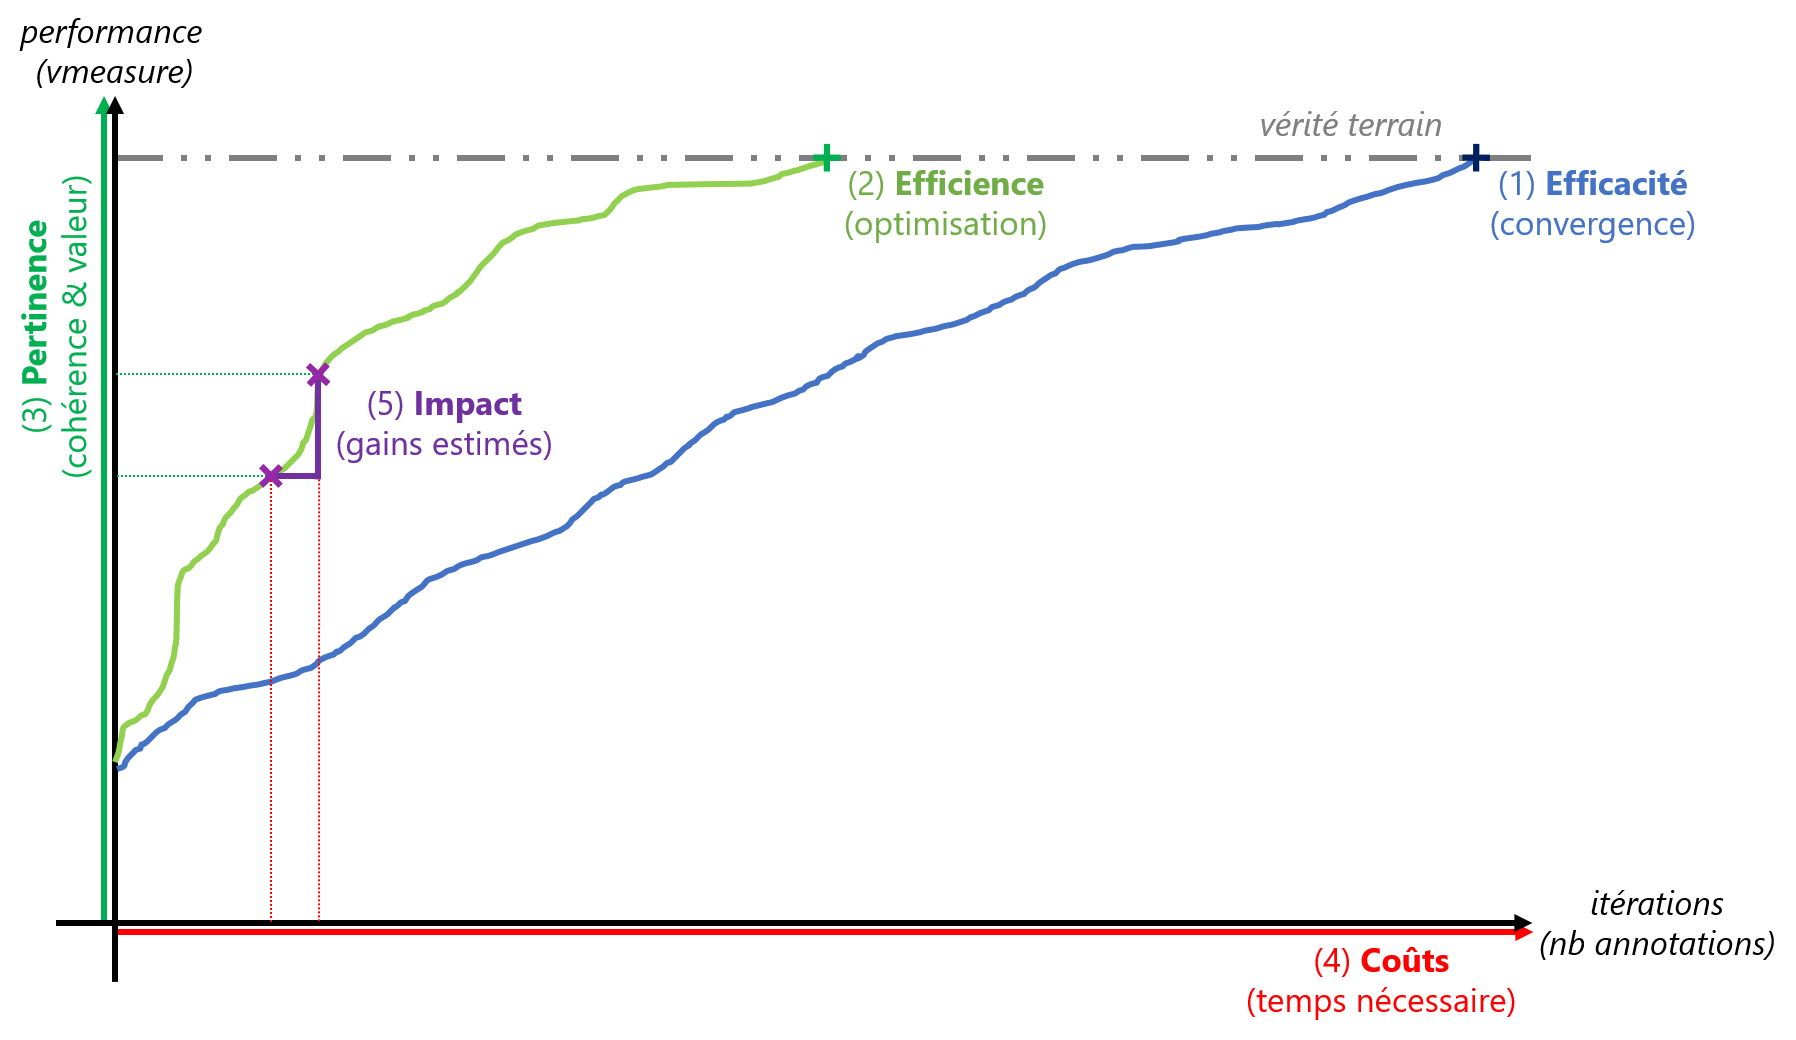
\includegraphics[width=0.8\textwidth]{figures/hypotheses-05-impact}
				\caption{Illustration des études réalisées sur le \textit{clustering} interactif (\textit{étape 5/6}) en schématisant l'évolution de la performance (\textit{v-measure par rapport à une vérité terrain}) d'une base d'apprentissage en cours de construction en fonction du nombre d'itérations de la méthode (\textit{nombre d'annotations}).}
				\label{figure:HYPOTHESE-IMPACT}
			\end{figure}

		\end{tcolorbox}
		
		%%%
		%%% Subsection 4.5.1: Étude d'estimation des cas d'arrêts de la méthode
		%%%
		\subsection{Étude d'estimation des cas d'arrêts de la méthode}
		
			%%% Protocole expérimental.
			\subsubsection{Protocole expérimental}
				\todo[inline]{Description succincte du protocole expérimental dans l'encadré d'hypothèse ?}

			%%% Résultats
			\subsubsection{Résultats obtenus}

			%%% Discussion
			\subsubsection{Discussion}
	

    %%%%%--------------------------------------------------------------------
    %%%%% Section 4.6: Hypothèse de robustesse.
    %%%%%--------------------------------------------------------------------
    \section{Hypothèse de robustesse : « \textit{quelle influence d'une erreur ?} »}
	\label{section:4.6-HYPOTHESE-ROBUSTESSE}
	
		%%% Formulation des hypothèses:
		Nous aimerions vérifier l'hypothèse de robustesse :
		\todo{à reformuler}

		\begin{tcolorbox}[
			title=\textbf{Hypothèse de robustesse},
			colback=gray!20,
			colframe=gray!50!black!75,
			width=\linewidth
		]
			« Il est possible d'\textbf{estimer l'influence d'une différence d'annotation} lors d'une méthodologie d'annotation basée sur le \textit{clustering} interactif (cf. figure~\ref{figure:HYPOTHESE-ROBUSTESSE}. »
			
			
			\begin{figure}[H]
				\centering
				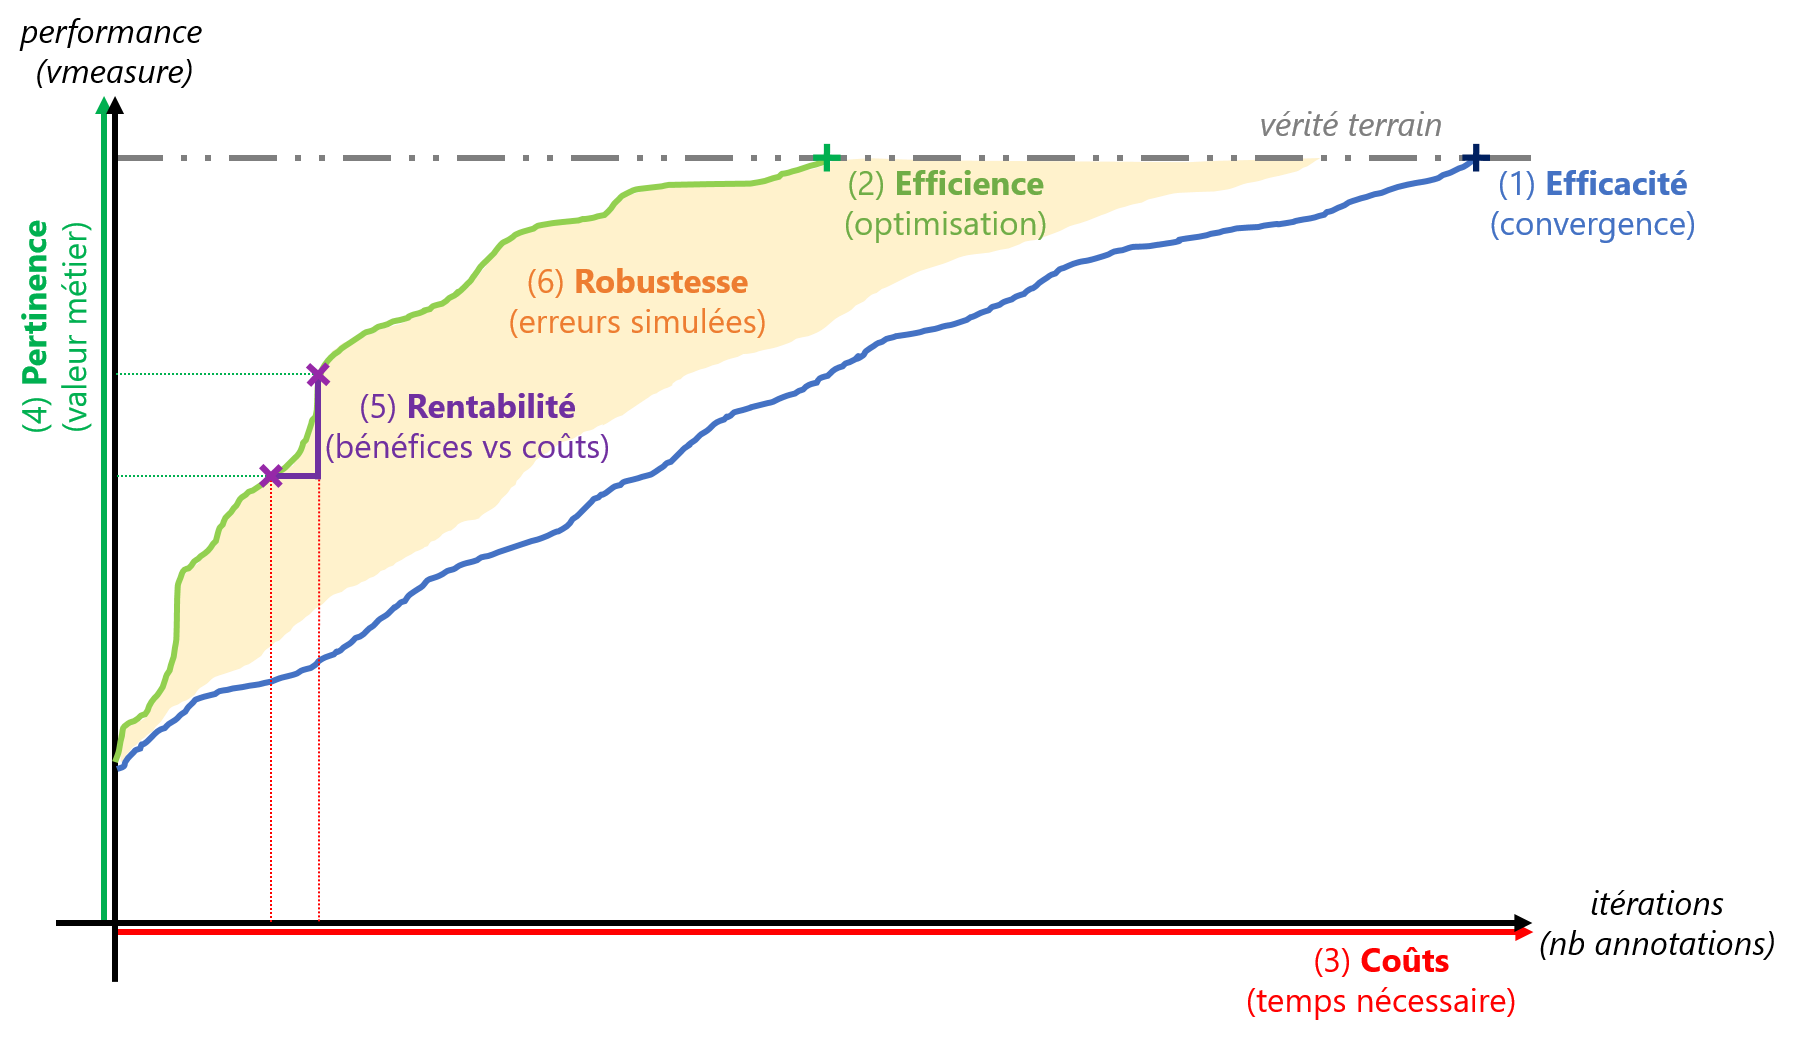
\includegraphics[width=0.8\textwidth]{figures/hypotheses-06-robustesse}
				\caption{Illustration des études réalisées sur le \textit{clustering} interactif (\textit{étape 6/6}) en schématisant l'évolution de la performance (\textit{v-measure par rapport à une vérité terrain}) d'une base d'apprentissage en cours de construction en fonction du nombre d'itérations de la méthode (\textit{nombre d'annotations}).}
				\label{figure:HYPOTHESE-ROBUSTESSE}
			\end{figure}

		\end{tcolorbox}
		
		%%%
		%%% Subsection 4.6.1: Étude de simulation d'erreurs d'annotations
		%%%
		\subsection{Étude de simulation d'erreurs d'annotations}
		
			%%% Protocole expérimental.
			\subsubsection{Protocole expérimental}
				\todo[inline]{Description succincte du protocole expérimental dans l'encadré d'hypothèse ?}

			%%% Résultats
			\subsubsection{Résultats obtenus}

			%%% Discussion
			\subsubsection{Discussion}
		
		%%%
		%%% Subsection 4.6.2: Étude d'annotation avec des paradigmes différents
		%%%
		\subsection{Étude d'annotation avec des paradigmes différents}
		
			%%% Protocole expérimental.
			\subsubsection{Protocole expérimental}
				\todo[inline]{Description succincte du protocole expérimental dans l'encadré d'hypothèse ?}

			%%% Résultats
			\subsubsection{Résultats obtenus}

			%%% Discussion
			\subsubsection{Discussion}
			
	
    %%%%%--------------------------------------------------------------------
    %%%%% Section 4.7:
    %%%%%--------------------------------------------------------------------
    \section{Autres études à réaliser}
	\label{section:4.7-ETUDES-DIVERSES}
	\todo[inline]{SECTION À RÉDIGER}

        \subsection{Choix du nombre de clusters ==> problème de recherche complexe}
            o	Piste de résolution : plusieurs clusterings + vote collaboratif ? algorithmes sans le nombre de clusters en hyper-paramètres

        \subsection{Impact d'un modèle de langage ==> nécessite de nombreuses données spécifiques au domaine}
            o	Piste de résolution : script d'étude comparative déjà prêt, mais il manque les données opensources… 

        \subsection{Paradigme d’annotation (intention vs dialogue) ==> problème d'UX + objectif métier}
            o	Etude Ergo, sort de mon domaine d'expertise

        \subsection{(et plein d'autres que j'ajouterai au fur et à mesure de ma rédaction)}
            o	
